The stability of the ten photodiodes used to survey the \laser~light is monitored with a LED signal. The light is also transmitted to a reference photodiode for normalization. This reference photodiode is itself monitor thanks to a radioactive source.\\
A view of the PHOCAL box is given on figure \ref{fig:lasphocal}. It is comprised of:
\begin{itemize}
\item LED box: houses the LED itself and an LED driver that provides a pulsed signal lasting 10 ns with an intensity that may be tweaked manually thanks to a potentiometer between 20 and 20 V.
\item reference box: 
\item Logic board:
\item optics fibers and light mixers
\end{itemize}


\begin{figure}[htbp]
\centering
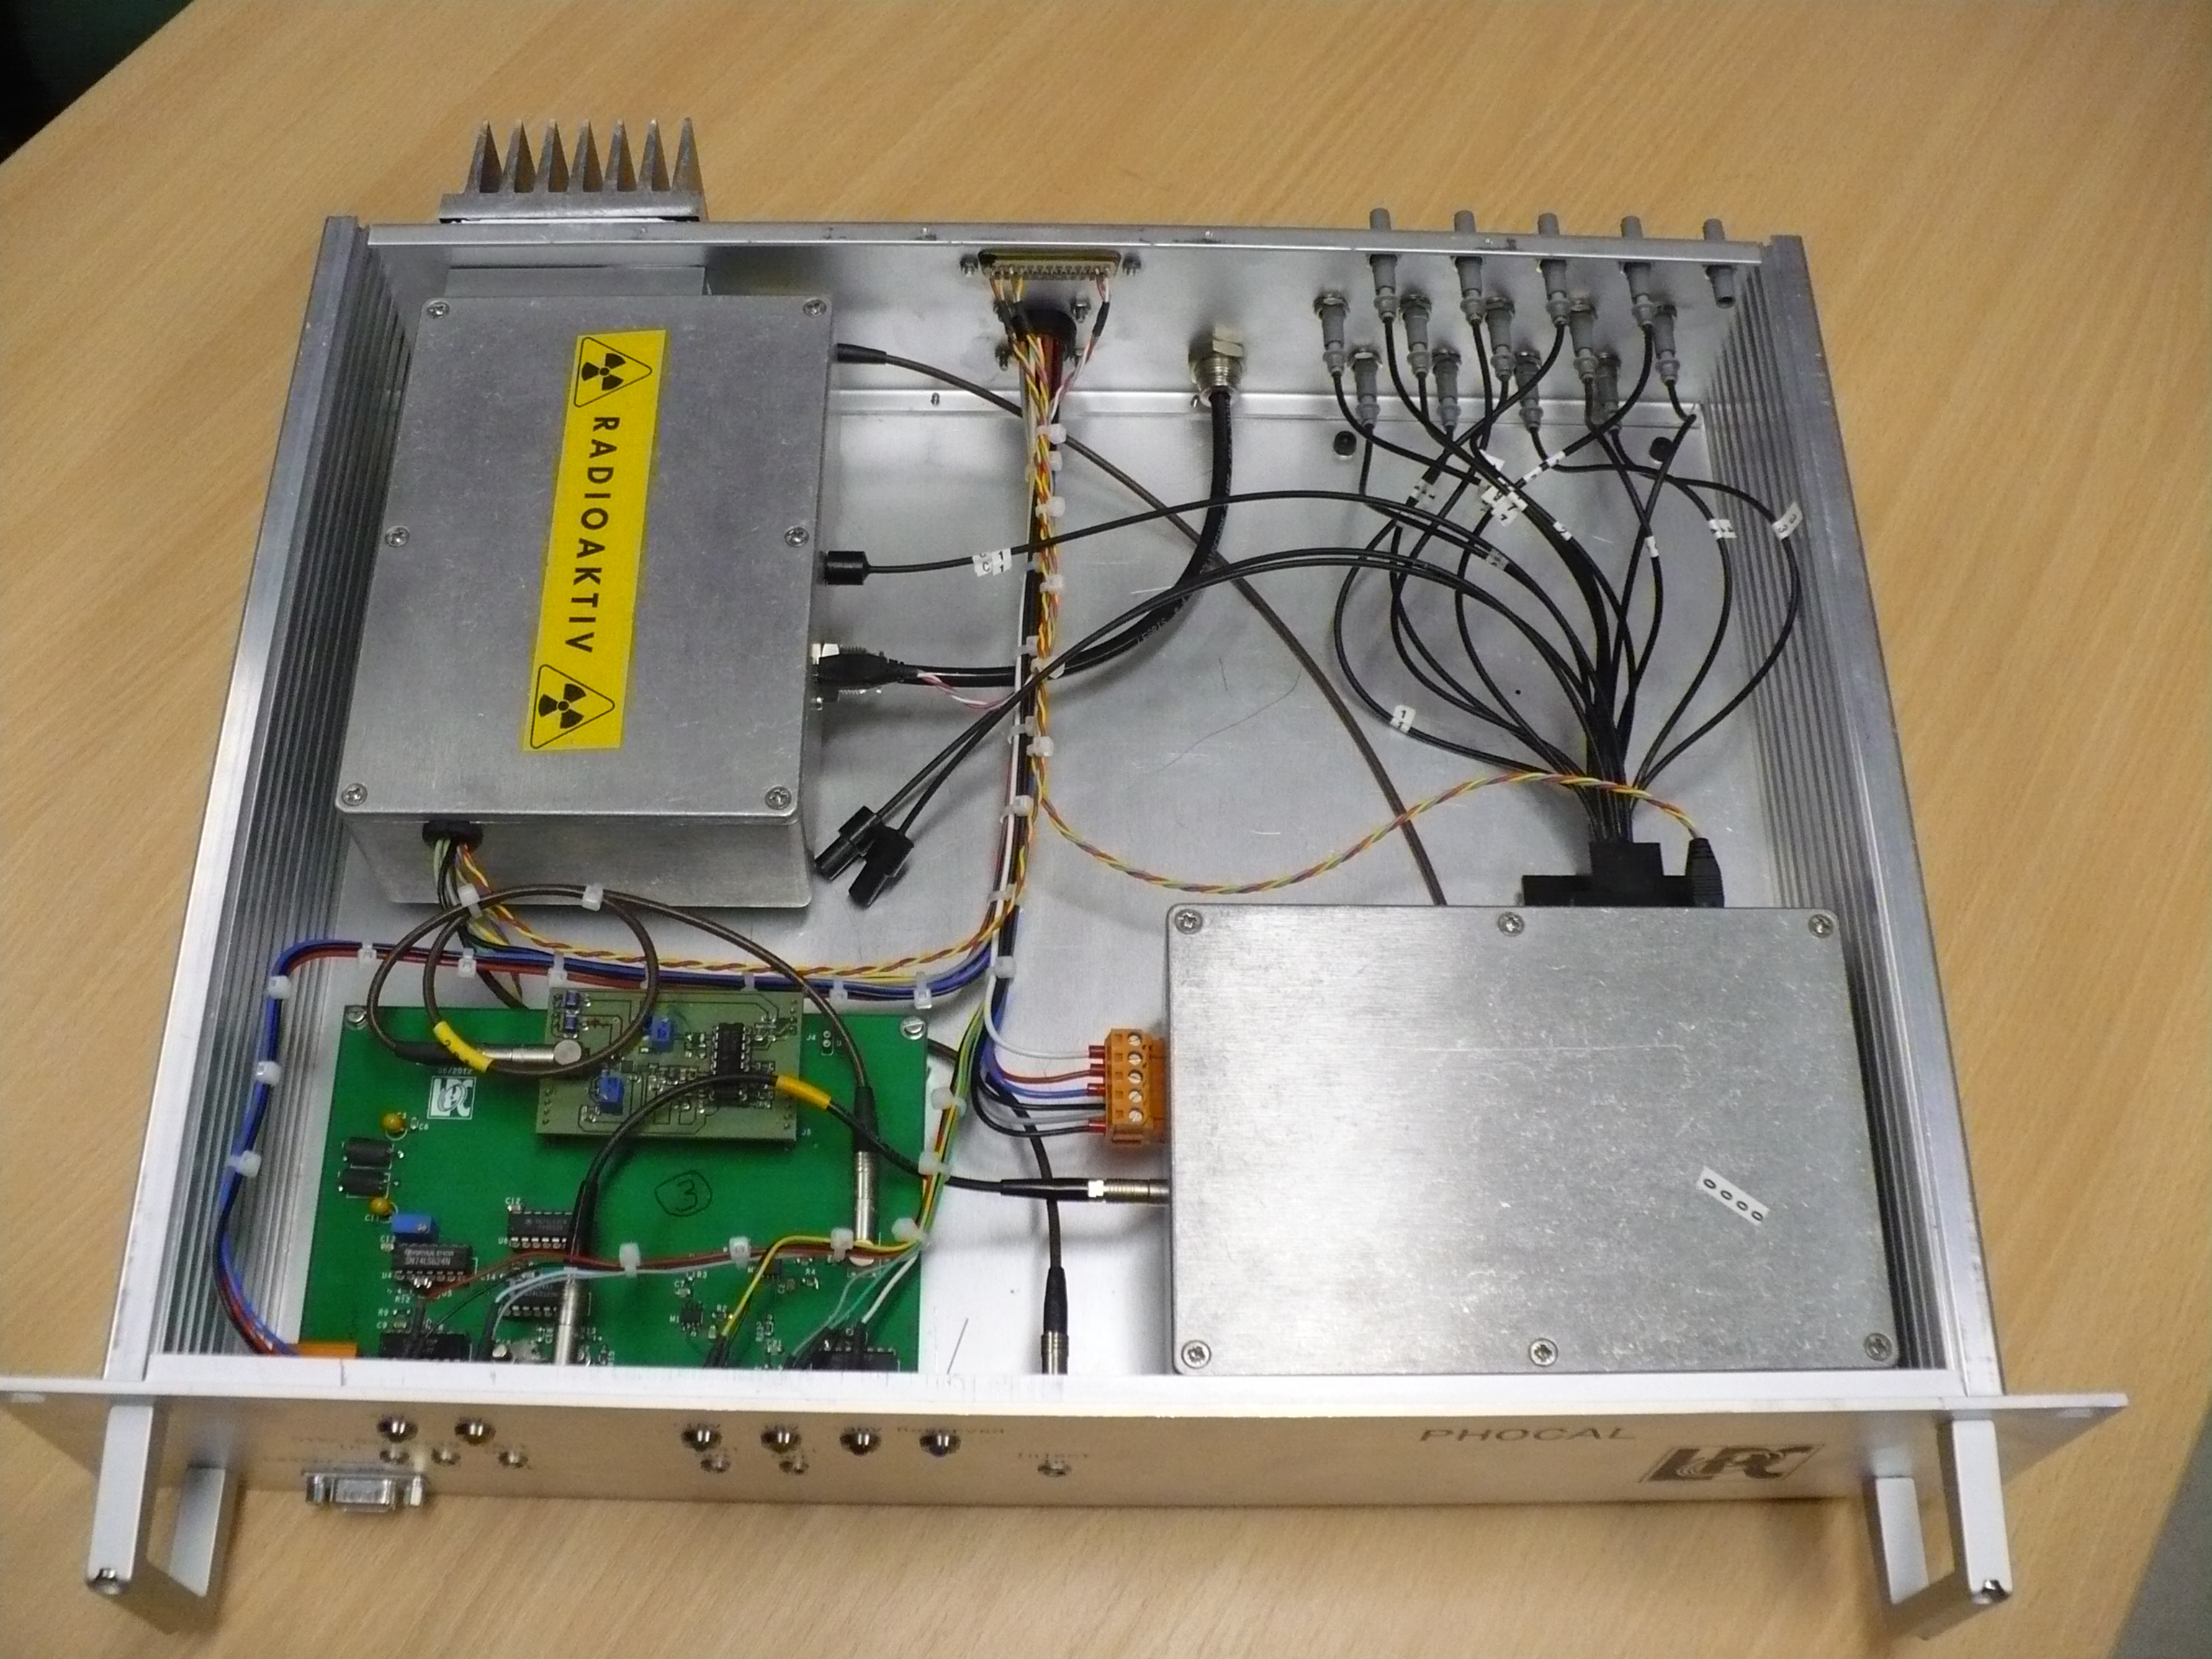
\includegraphics[height=6cm]{figures/phocal1.JPG}
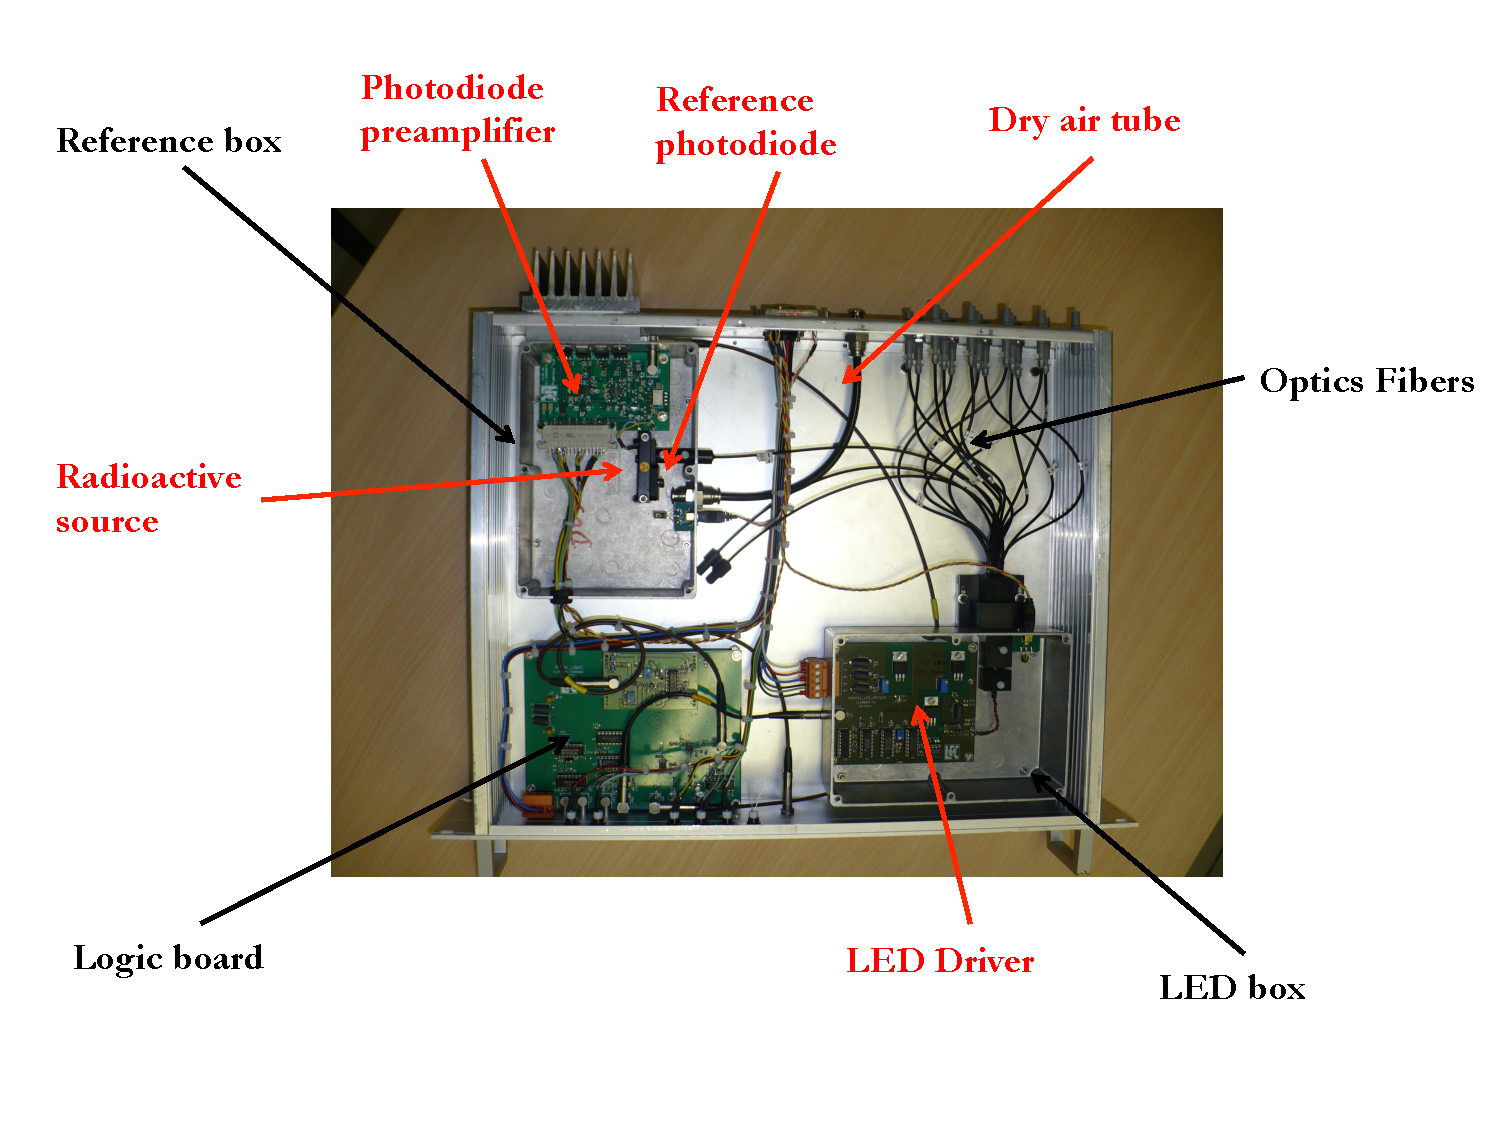
\includegraphics[height=10cm]{figures/phocal2_comm.pdf}
\caption{View of the PHOCAL system}\label{fig:lasphocal}
\end{figure}